%% ============================================================
%% 分片 29：原文第 10 节「The Bogomolny Equations And The Space Of Hecke Modifications」（原文 glshort.tex 起于第 8120 行）
%% 由 tools/harvmac2tex.py 从 arXiv 源码（hep-th/0604151v3）自动生成。
%% 只译英文散文；公式、编号、\label、\cite 一律不改。
%% ============================================================

\subsection{'t Hooft 算子的算子乘积展开}

\label{sec:opprod}

让我们把 $^L\negthinspace G$ 的表示的张量积写成
% 式 (10.21)
\setcounter{equation}{20}
\begin{equation}\label{eq:yurgo}
^L\negthinspace R\otimes {}^L\negthinspace
R'=\bigoplus_{\alpha\in \EUR}\left(N_\alpha \otimes{}^L\negthinspace R_\alpha\right).
\end{equation}

这里 $N_\alpha$ 是向量空间 $N_\alpha={\rm Hom}_G({}^L\neg R\otimes {}^L\neg{R'},{}^L\neg R_\alpha)$，其中 ${\rm Hom}_G$ 指 $G$-不变线性变换构成的空间。集合 $\EUR$ 由那些使 $N_\alpha$ 非零的表示组成。为方便起见，我们还用 $n_\alpha$ 记向量空间 $N_\alpha$ 的维数这个整数。

正如我们在第~\ref{sec:lineop}~节所讨论的，表示的张量积恰好反映在 Wilson 算子的算子乘积展开中。在式~\eqref{eq:tryo} 中，我们用 $c$-数系数 $n_\alpha$ 写出了 Wilson {\it 圈}算子的算子乘积展开。然而，对于静态 Wilson {\it 线}算子——我们把它视为量子化问题的一部分，而不是作用在量子态上的算子——可以写出一个密切相关且更精确的陈述：
% 式 (10.22)
\setcounter{equation}{21}
\begin{equation}\label{eq:docus}
W({}^L\neg R,p)\cdot W({}^L\neg\tilde R,p')\to
\bigoplus_{\alpha\in\EUR}\left(N_\alpha\otimes W({}^L\neg
R_\alpha,p')\right).
\end{equation}

这里我们取规范群为 $^L\neg G$，$p$ 与 $p'$ 是静态 Wilson 算子的位置。\eqref{eq:docus}\ 给出了如下构造的方子：在带有标号为 $^L\neg R$ 与 $^L\neg R'$ 的两个 Wilson 算子时，量子 Hilbert 空间是若干贡献的直和；每一份贡献是在带有一个标号为 $^L\neg R_\alpha$ 的 Wilson 算子时量子化所得量子 Hilbert 空间与向量空间 $N_\alpha$ 的张量积。\eqref{eq:docus}\ 的依据是：在量子理论中，静态 Wilson 算子的效果是引入相应表示中的外源电荷。若有两个静态 Wilson 算子，就有两个外源电荷；把相应表示的张量积分解为不可约表示的直和之后，就得到 \eqref{eq:docus}。

由 $S$-对偶，我们预期 't Hooft 线算子的相应算子乘积展开取同样的形式
% 式 (10.23)
\setcounter{equation}{22}
\begin{equation}\label{eq:zurgo}
T({}^L\negthinspace R,p)\cdot T({}^L\negthinspace
R',p')\to \bigoplus_{\alpha\in \EUR}\left(N_\alpha \otimes T({}^L\negthinspace
R_\alpha,p')\right).
\end{equation}

正如第~\ref{sec:lineop}~节那样，即使不用 $S$-对偶，由于在 $\Psi=0$ 处 't Hooft 算子是唯一的线算子，像 \eqref{eq:zurgo}\ 这样的关系必须以某个表示集合 $\EUR$（它依赖于 $^L\negthinspace R$ 与 $^L\negthinspace R'$）以及某些向量空间 $N_\alpha$ 成立。此外，用简单的论证就足以确定集合 $\EUR$，它依赖于 $^L\negthinspace R$ 与 $^L\negthinspace R'$。所以问题在于描述 $N_\alpha$。

若专门考虑普通的、可以作用在量子态上的 't Hooft 圈算子（相对于会改变量子 Hilbert 空间定义的静态线算子），则算子乘积展开中的系数是普通的 $c$-数 $n_\alpha$，而不是向量空间 $N_\alpha$。实现这种专门化的一种办法是把「时间」方向取成一个圆。这样会对所有量子 Hilbert 空间取迹，向量空间 $N_\alpha$ 便换成了它的整数维数 $n_\alpha$。静态 't Hooft 线算子变成环形的 't Hooft 圈算子（如果改把另一个方向解释为量子化的「时间」方向，它就能作用在量子态上），于是我们得知：'t Hooft 圈算子、乃至拓扑场论中任何圈算子的算子乘积展开系数都是整数。

换一种略有不同的说法，让我们回到 Wilson 算子的情形。闭合 Wilson 圈算子通过和乐（holonomy）的迹来定义。取迹把向量空间换成了它的维数。而开 Wilson 算子（对我们重要的例子是静态 Wilson 线算子）用和乐本身来定义，即把它看作某个向量空间上的算子。在分解这类算子的张量积时，「系数」是向量空间 $N_\alpha$，而非整数 $n_\alpha$。就某些目的而言，这一区别并不重要，可以把 $N_\alpha$ 换成它的维数。

\par\medskip{\it 一些有用的膜}

一旦把场景布置妥当，$N_\alpha$ 的确定便是一门数学理论的推论。这门理论发端于 Lusztig 的工作 \cite{ref98}，它把 $G$ 的不可约表示张量积中的重数与 $^L\neg G$ 上仿射 Schubert 簇的相交上同调复形（intersection cohomology complexes）的卷积联系起来；后经 Ginzburg \cite{ref96} 以及 Mirkovic 与 Vilonen \cite{ref97} 提炼为张量范畴的等价。用物理语言说，这一提炼关乎 't Hooft 算子乘积展开的一种描述：其中「系数」是向量空间 $N_\alpha$（如我们的式~\eqref{eq:zurgo}），而不是更传统的、只考虑闭环算子并把 $N_\alpha$ 换成其整数维数 $n_\alpha$ 的描述（如我们的式~\eqref{eq:tryo}）。我们将先为分析搭好框架，在不借助数学的情况下尽可能用纯物理推理推进，然后再尝试阐明相应的数学理论。

\begin{figure}[htbp]
\centering
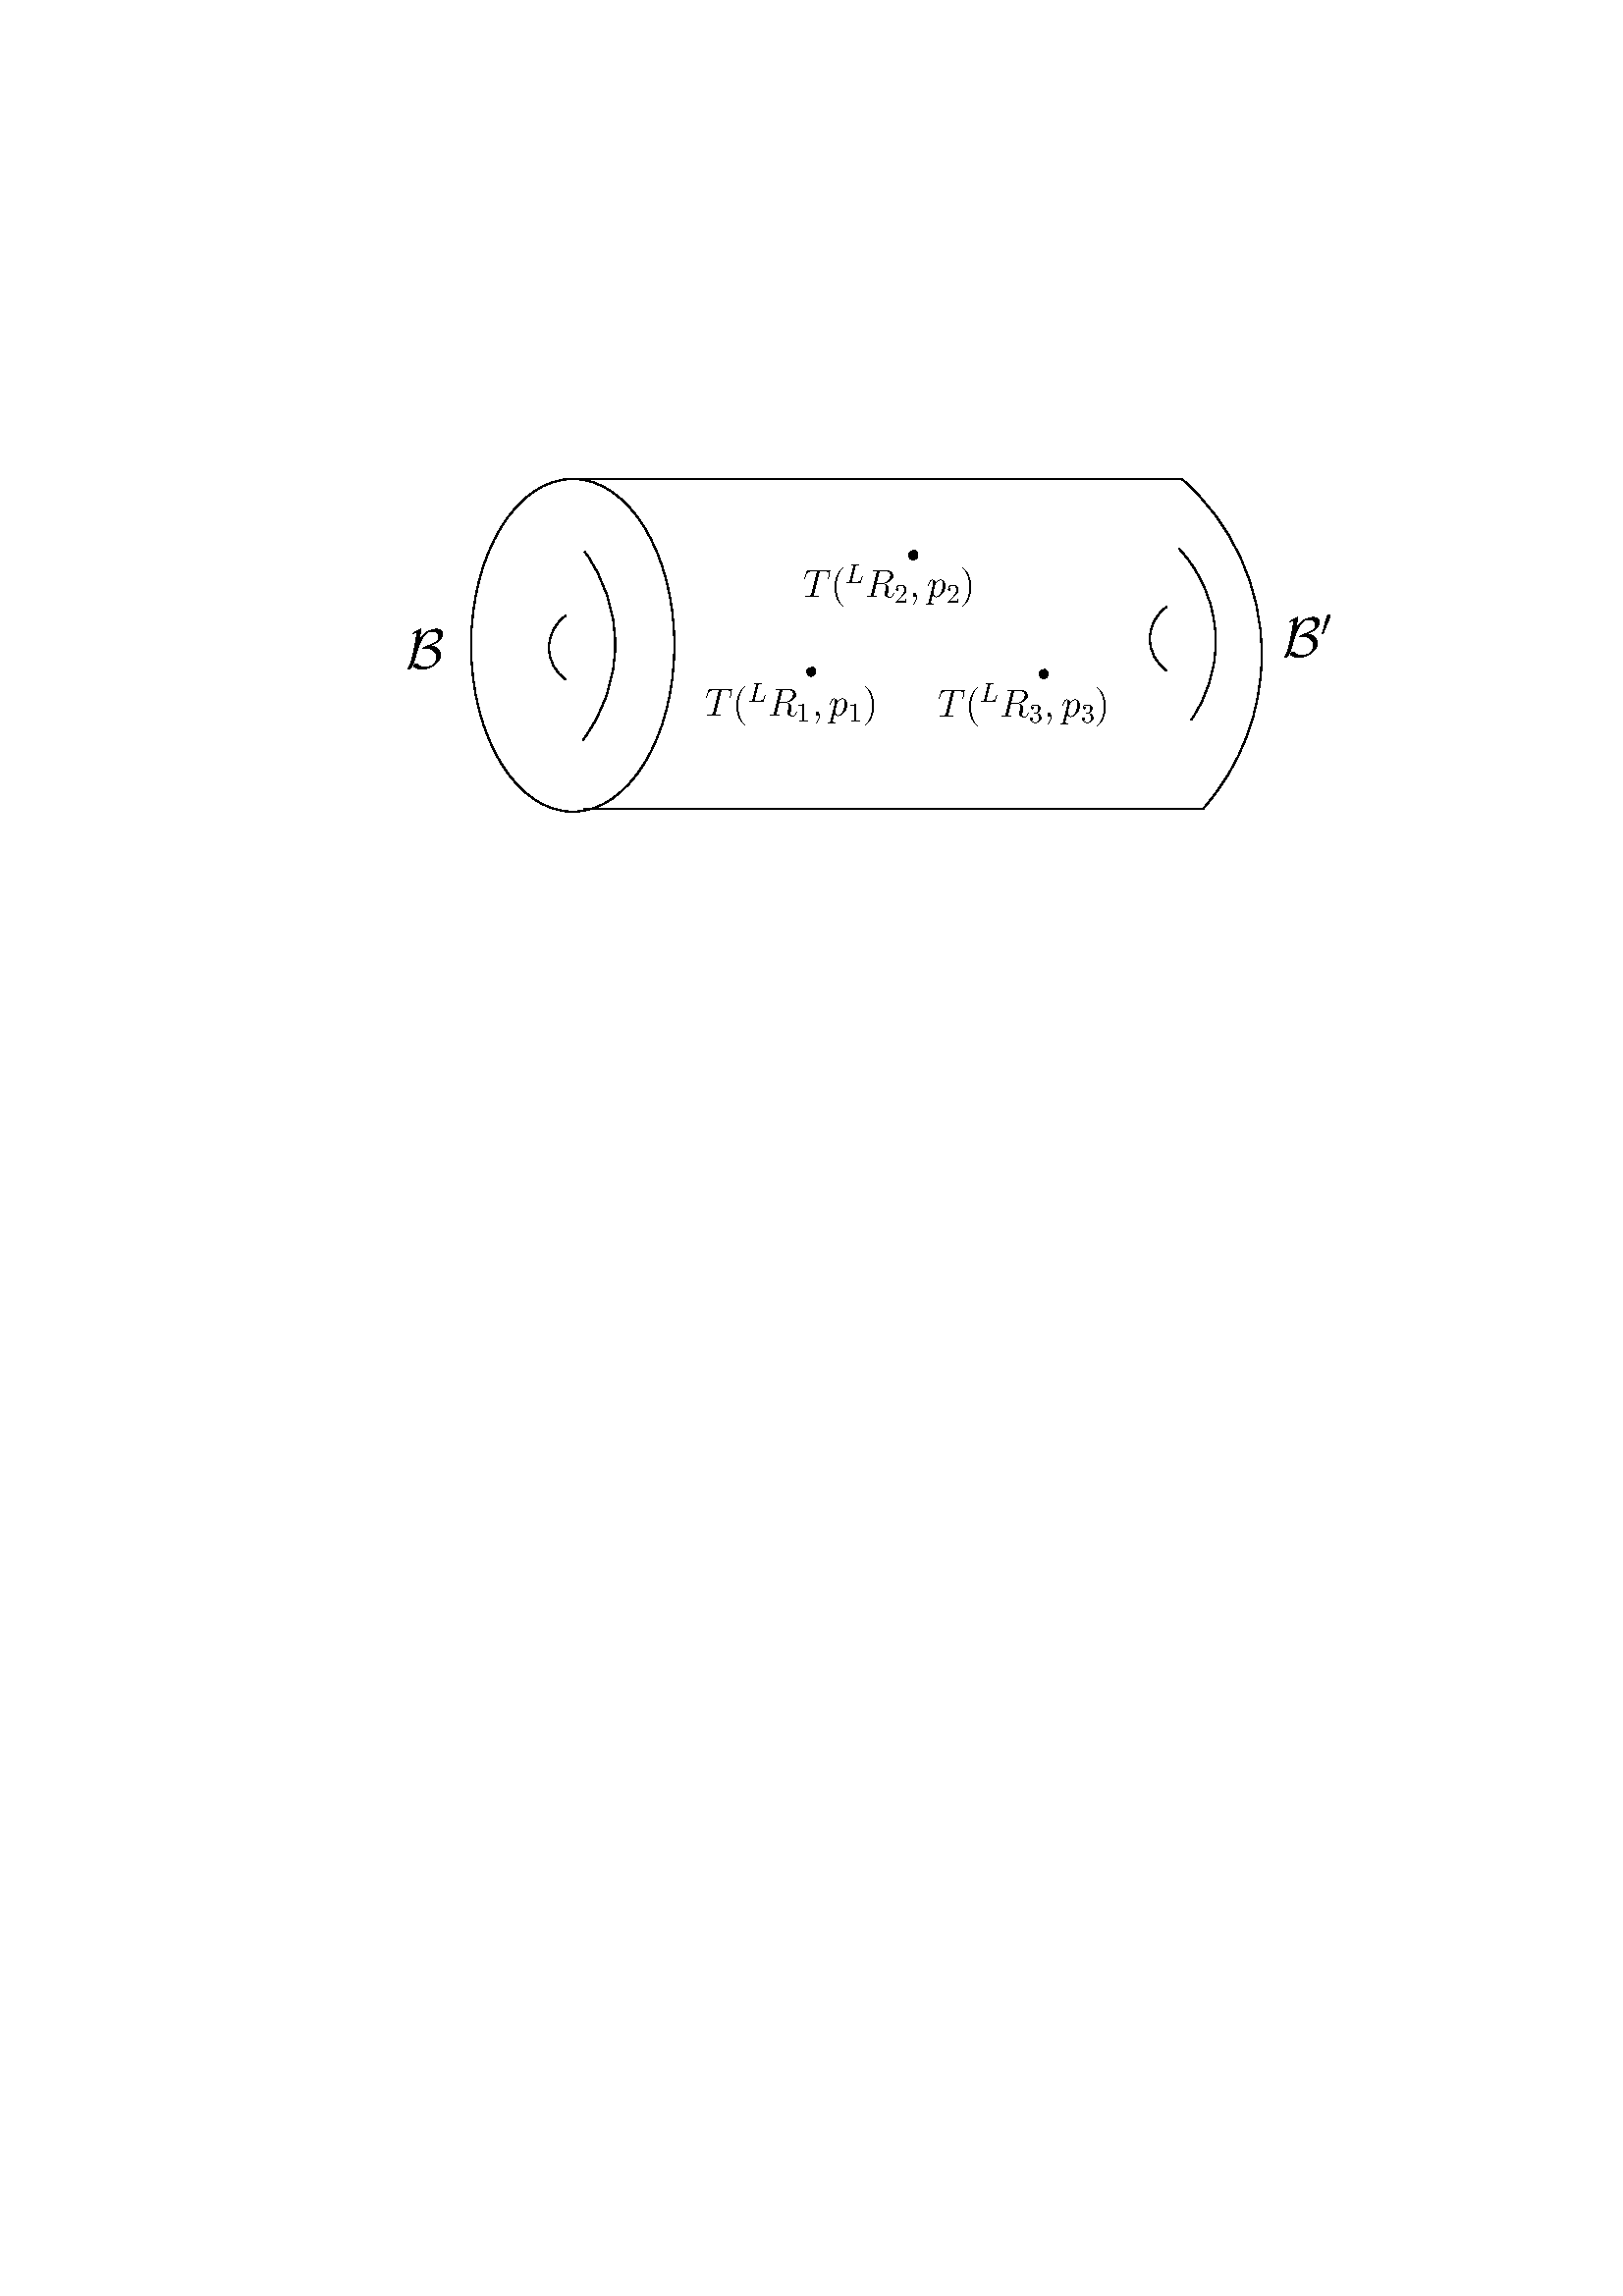
\includegraphics[width=0.75\linewidth]{figures/gla7-8.png}
\caption{Insertion of several 't Hooft operators $T({}^L\negthinspace R_i,p_i)$, with a brane ${\cal B}$ on the left that specifies an ``initial'' bundle $E_-$, and a brane ${\cal B}'$ on the right that sets $\varphi=0$.（原文 Fig.~19）}
\label{fig:xitampo}
\end{figure}

 要确定 $N_\alpha$，只需考虑任意一类方便且足够丰富的、其中静态 't Hooft 算子起作用的计算即可。为此，我们在熟悉的三维流形 $W=I\times C$ 中考虑两个或更多 't Hooft 算子，并在两端选取适当的膜 ${\cal B}$ 与 ${\cal B}'$。我们希望选取那些能使计算简化的膜。

't Hooft 算子保持 $(B,A,A)$ 型超对称，因此最自然的是取 ${\cal B}$ 与 ${\cal B}'$ 为该类型的膜。为此，我们可以取 ${\cal B}$ 与 ${\cal B}'$ 的支撑为 Hitchin 模空间 $\MH$ 中的子簇 $U$ 与 $U'$，它们在复结构 $I$ 中全纯，并且相对于该复结构中为 $(2,0)$ 型的辛形式 $\Omega_I$ 是拉格朗日的。（简言之，$U$ 与 $U'$ 是复结构 $I$ 中的复拉格朗日子流形。）我们给 $U$ 与 $U'$ 配上平凡的 Chan-Paton 线丛。

我们取 $U$ 参数化 Hitchin 对 $(E,\varphi)$，其中要求 $E$ 具有指定的全纯型 $E_-$，而 $\varphi$ 任意。我们要求 $E_-$ 稳定，除此之外 $E_-$ 的选取无关紧要。再取 $U'$ 参数化对 $(E,0)$，其中 $E$ 任意而 $\varphi=0$。

第一点是：$U$ 与 $U'$ 横截相交于唯一一点，对应于 Higgs 丛 $(E_-,0)$。此外，$U$ 与 $U'$ 是复结构 $I$ 中的复辛流形，故 ${\cal B}$ 与 ${\cal B}'$ 是 $(B,A,A)$ 型膜。

最后，我们这样选取 ${\cal B}$ 与 ${\cal B}'$：带这些边界条件、并包含某些 't Hooft 算子时，超对称位形构成的空间恰好就是熟悉的 Bogomolny 方程解的模空间 ${\EUZ}({}^L\negthinspace R_1,p_1;\dots;{}^L\negthinspace R_k,p_k)$。

这个陈述涉及几处微妙之处。首先，超对称位形一般有 $\varphi\not= 0$，必须用第~\ref{sec:thooftheckeop}~节开头描述的扩展 Bogomolny 方程而非普通 Bogomolny 方程来描述。我们甚至还没有分析过扩展 Bogomolny 方程；那将是第~\ref{sec:extbog}~节的主题。到时候我们会看到：若 $\varphi$ 在 $W$ 的一端为零——由于 $U'$ 的选取，这里正是如此——则 $\varphi$ 处处为零，扩展 Bogomolny 方程约化为普通方程。

其次，在描述膜 ${\cal B}$ 与 ${\cal B}'$ 时，我们只描述了以 $\MH$ 为目标的 sigma 模型各场 $(A,\varphi)$ 的边界条件。场 $\phi_0$ 是 Bogomolny 方程的重要组成部分，它出现在规范理论中，却不出现在 sigma 模型中（除奇点处外），因为约化到二维时它是「有质量」的。把第~\ref{sec:zapendix}~节的分析加以推广，可以在规范理论中同时描述膜 ${\cal B}$ 与 ${\cal B}'$ \cite{ref26}，而在那个框架里可以证明：场 $\phi_0$ 的恰当边界条件正是我们所采用的那些。

\par\medskip{\it 物理态的空间}

在 $A$-模型中，没有瞬子修正时（这里不存在瞬子修正，原因见第~\ref{sec:thooftheckeop}~节开头），物理态的空间是时间无关超对称位形空间的上同调。事实上，从物理上理解的 $A$-模型最自然地给出 de Rham 上同调。

换句话说，在膜 ${\cal B}$ 与 ${\cal B}'$ 以及 't Hooft 算子 $T(^L\negthinspace R_i,p_i)$ 之下，物理态的空间就是我们熟悉的、带适当奇点的 Bogomolny 方程解模空间 $\bar\EUZ(^L\negthinspace R_1,p_1;\dots;^L\neg R_k,p_k)$ 的上同调。由于 $\bar\EUZ$ 一般有奇点，这里需要说明所谓的 de Rham 上同调究竟指何种改进。但首先让我们形式地陈述所期待的结果是什么样子。

对每个有限表示集 $^L\negthinspace R_i$（$i=1,\dots,k$），模空间 $\bar\EUZ=\bar\EUZ(^L\negthinspace R_1,p_1;\dots;{}^L\neg R_k,p_k)$ 的上同调给出一个物理态空间 ${\cal H}({}^L\negthinspace R_1,{}^L\negthinspace R_2,\dots,{}^L\negthinspace R_k)=H^*(\bar\EUZ)$。注意，由于底层的四维拓扑场论（TQFT），点 $p_i$ 的选取无关紧要。更确切地说，TQFT 表明：在 $p_i$ 的局部，物理态空间与 $p_i$ 无关（在不同点 $p_i$ 构成的空间上有平坦联络\footnote{移动这些点是改变 $W$ 上度规的特殊情形。度规的改变在 BRST 上同调中是平凡的，这一事实给出该平坦联络。}）。由于三维流形 $W=I\times C$ 中的 $n$ 元组空间是单连通的，也不会有单值性，因此 $p_i$ 无关紧要。所以我们只用表示、而不用点，把物理态空间记为 ${\cal H}({}^L\negthinspace R_1,\dots,{}^L\negthinspace R_k)$。

除开关于奇点的问题，这个论证其实并不需要量子场论。当表示 $^L\negthinspace R_i$ 极小（且 $p_i$ 互异）时，$\bar\EUZ(^L\negthinspace R_1,p_1;\dots;{}^L\neg R_k,p_k)$ 是一族光滑流形。这样一族流形的上同调是局部常值的，正如 TQFT 所预期。在带奇点的一般情形，我们必须确保使用一种能保证这类论证成立的 de Rham 上同调的改进。使这一点成为可能的性质是：$\bar\EUZ(^L\negthinspace R_1,p_1;\dots;{}^L\neg R_k,p_k)$ 虽有奇点，但其奇点结构完全与 $p_i$ 无关。奇点来自单个 Hecke 变换的退化（或单个 't Hooft 算子位置处的单极子冒泡），与其他算子的位置无关。

现在，算子乘积展开说我们可以把 't Hooft 算子的乘积 $T(^L\negthinspace R_1)\cdot T(^L\negthinspace R_2)$ 换成和 $\oplus_{\alpha\in \EUR}C_\alpha\otimes T(^L\negthinspace R_\alpha)$，其中 $\EUR$ 是某个集合，$C_\alpha$ 是某些向量空间。在目前的语境下——针对我们所考虑的膜存在时的物理态空间——这意味着必须有一族同构 % 式 (10.24)
\setcounter{equation}{23}
\begin{equation}\label{eq:mitrox}
{\cal
H}({}^L\negthinspace R_1,{}^L\negthinspace
R_2,\dots,{}^L\negthinspace R_k)\cong\oplus_{\alpha\in
\EUR}\left(C_\alpha \otimes{\cal H}({}^L\negthinspace
R_\alpha,{}^L\negthinspace R_3,\dots,{}^L\negthinspace R_k)\right).
\end{equation}

由于左端只依赖于表示构成的无序集合 $^L\negthinspace R_i$，\eqref{eq:mitrox}\ 中的同构自动与结合律相容，也就是与「反复取算子乘积以进一步减少表示数目」相容。

$S$-对偶表明：集合 $\EUR$ 与向量空间 $C_\alpha$ 应当就是 $^L\negthinspace R$ 的表示张量积中出现的那一组：
% 式 (10.25)
\setcounter{equation}{24}
\begin{equation}\label{eq:omigron}
^L\negthinspace R_1\otimes {}^L\negthinspace
R_2=\oplus_{\alpha\in \EUR}\left(N_\alpha\otimes{} ^L\negthinspace R_\alpha\right).
\end{equation}

其实我们可以更具体一些，只要回忆起\footnote{这些断言与点 $p_i\in W$ 无关，故略去。}：${\cal H}({}^L\negthinspace R_1,^L\negthinspace R_2,\dots,^L\negthinspace R_k)$ 是 $\bar\EUZ({}^L\negthinspace R_1,{}^L\negthinspace R_2,\dots,{}^L\negthinspace R_k)$ 的上同调，而且从拓扑上看 $\bar\EUZ({}^L\negthinspace R_1,{}^L\negthinspace R_2,\dots,{}^L\negthinspace R_k)$ 就是简单乘积 $\prod_{i=1}^k\bar\EUZ({}^L\negthinspace R_i)$。（而 $\bar\EUZ({}^L\negthinspace R_i)$ 等同于 ${}^L\negthinspace R_i$ 型 Hecke 修正的紧化空间 $\bar {{\EUY}}({}^L\negthinspace R_i)$。）乘积的 de Rham 上同调是各因子上同调之积，于是得到 % 式 (10.26)
\setcounter{equation}{25}
\begin{equation}\label{eq:kipro}
{\cal H}({}^L\negthinspace
R_1,{}^L\negthinspace R_2,\dots,{}^L\negthinspace
R_k)=\otimes_{i=1}^k {\cal H}({}^L\negthinspace R_i).
\end{equation}
 这意味着 \eqref{eq:mitrox}\ 必定真正来自一族同构 % 式 (10.27)
\setcounter{equation}{26}
\begin{equation}\label{eq:gitrox}
{\cal H}({}^L\negthinspace R_1)\otimes
{\cal H}({}^L\negthinspace R_2)=\oplus_{\alpha\in \EUR}N_\alpha\otimes
{\cal H}({}^L\negthinspace R_\alpha).
\end{equation}

把 \eqref{eq:omigron}\ 与 \eqref{eq:gitrox} 相比较，我们看到 ${\cal H}({}^L\negthinspace R_i)$ 服从与 $^L\negthinspace R_i$ 相同的张量积代数。这提示存在 ${\cal H}({}^L\negthinspace R_i)$ 与 $^L\negthinspace R_i$ 之间的同构，它给出两个代数之间的自同构。事实上，可以证明 \cite{ref127}：对于有限维向量空间族 $^L\negthinspace R_i$ 与 ${\cal H}(^L\negthinspace R_i)$ 来说，这是它们具有相同张量积代数的唯一途径。${\cal H}({}^L\negthinspace R_i)$ 与 $^L\negthinspace R_i$ 之间的同构在相差 $^L\negthinspace G$ 中元素的共轭意义下唯一。

\par\medskip{\it 按鬼数分次}

由于 $^L\negthinspace G$ 当然以一种与张量积相容的方式作用在 $^L\negthinspace R_i$ 上，这意味着 $^L\negthinspace G$ 也相应地作用在 ${\cal H}({}^L\negthinspace R_i)$ 上（在相差共轭意义下定义）。从物理观点看，这意味着什么是神秘的，因为在 $\Psi=0$ 处 $^L\negthinspace G$ 并不是规范群为 $G$ 的整个 $A$-模型的对称性，而只是我们为分析算子乘积展开所考察的那一小块的对称性。（如果能理解构造中所用膜 ${\cal B}$ 与 ${\cal B}'$ 的 $S$-对偶，事情也许会变得更清楚。）然而，整个 $A$-模型确实有一个相关的对称性。

这就是「鬼数」对称性 ${\EUK}$，它在 ${\EUN}=4$ 超对称杨–米尔斯理论的拓扑扭化中的起源已在第~\ref{sec:twisting}~节解释过。在 $A$-模型中，鬼数粗略地说就是上同调类的次数或维数。\footnote{对 Kähler 目标，Hodge 分解 $H^d(X)=\oplus_{p+q=d}\,H^{p,q}(X)$ 一般会给出 $A$-模型的进一步精细化。然而这与我们目前的讨论无关，因为空间 $\bar \EUZ({}^L\negthinspace R_1,\dots,{}^L\neg R_k)$ 的上同调全为 $(p,p)$ 型。}不过，有一处关键的微妙之处。对复维数为 $n$ 的复流形 $X$，微分形式的次数通常理解为从 $0$ 取到 $2n$。但 $A$-模型的物理态空间有一个费米子共轭对称性\footnote{这里所说的对称性是二维 CPT 对称性。它是具有 $(2,2)$ 超对称、目标为 $X$ 的物理超对称 sigma 模型的精确对称性。在非平坦 Riemann 面 $\Sigma$ 上，这一对称性会被定义 $A$-模型的拓扑扭化破坏。但物理态空间是在平坦流形 $\Bbb{R}\times S^1$ 上量子化 sigma 模型得到的，不受该扭化影响。}，它把维数为 $d$ 的类与维数为 $2n-d$ 的类互换，并把 ${\EUK}\to -{\EUK}$。与次数为 $d$ 的上同调类相应的态，其鬼数实际上是\footnote{为完整起见，我们指出：若 $X$ 是 Calabi-Yau 流形，则 $A$-模型中从态到算子的映射涉及一个谱流，它给 ${\EUK}$ 加上 $\dim_{\Bbb{C}}(X)$。因此若 $\psi$ 是 $X$ 的 $d$ 维上同调中的一个类，则对应于 $\psi$ 的 $A$-模型态满足 ${\EUK}=d-{\rm dim}_{\Bbb{C}}(X)$，而相应的算子 ${\EUO}_\psi$ 满足 ${\EUK}=d$。然而空间 $\bar \EUZ({}^L\negthinspace R_1,\dots,{}^L\neg R_k)$ 并非 Calabi-Yau，更重要的是，我们关于膜与 't Hooft 算子的讨论针对的是物理态，而非相应的算子。} % 式 (10.28)
\setcounter{equation}{27}
\begin{equation}\label{eq:insno}
{\EUK}=d-{\rm dim}_{\Bbb{C}}(X).
\end{equation}

在从 $^L\negthinspace R_i$ 到 ${\cal H}(^L\negthinspace R_i)$ 的映射中，$A$-模型的对称性 ${\EUK}$ 必须对应于 $^L\negthinspace G$ 的表示张量代数的一个导子（即某个自同构的生成元）。任何这样的导子实际上都是复化李代数 $^L\negthinspace \frak{g}$ 的元素。对应于 ${\EUK}$ 的 $^L\negthinspace \frak{g}$ 元素在相差共轭意义下是良定义的。

对给定的 $^L\negthinspace G$，可以通过考察一个具体例子来找出正确的共轭类。例如，对 $^L\negthinspace G=SU(N)$，考虑 $N$ 维表示 $\VV$。相应的 Hecke 修正空间是 $\bar {{\EUY}}(\VV)\cong \Bbb{CP}^{N-1}$，正如我们在第~\ref{sec:spaceheck}~节所学到的。$\Bbb{CP}^{N-1}$ 的 de Rham 上同调是 $N$ 维的。这一维数与 $\VV$ 的维数相符，正是对应 $^L\negthinspace R\leftrightarrow {\cal H}({}^L\negthinspace R)$ 的一个例子。$\Bbb{CP}^{N-1}$ 的复维数为 $N-1$，其非零上同调出现在次数 $d=0,2,4,\dots,2N-2$。所以对应于 ${\EUK}$ 的 $^L\negthinspace \frak{g}$ 元素在表示 $\VV$ 中的本征值为 $N-1,N-3,N-5,\dots,-(N-1)$： % 式 (10.29)
\setcounter{equation}{28}
\begin{equation}\label{eq:unosn}
\EUK=\left(\begin{matrix}N-1& &&& \\ & N-3 &&&\\ &&
N-5 &&\\ &&&\ddots & \\ &&&& -(N-1)\\\end{matrix}\right).
\end{equation}
 对 $^L\negthinspace G=SU(2)$，${\EUK}$ 的共轭类就是 % 式 (10.30)
\setcounter{equation}{29}
\begin{equation}\label{eq:mitlgo}
{\EUK}\cong\left(\begin{matrix}1 & 0 \\ 0 & -1
\\\end{matrix}\right).
\end{equation}

\par\medskip{\it 相交上同调}

一门由 Lusztig 开创 \cite{ref98}、后经 Ginzburg \cite{ref96} 以及 Mirkovic 与 Vilonen \cite{ref97} 提炼的数学理论，实际上确定了 't Hooft 算子乘积展开中的「系数」。详述这些结果的任务最好留给别人。作为替代，我们在此尝试用物理学家可能觉得有启发的语言表达其中一些想法。


首先，该定理所用的上同调理论是相交上同调 \cite{ref128,ref129}。粗略地说，并在标准猜想成立的前提下，代数簇 $X$ 的相交上同调就是 $X$ 光滑部分的 ${\Bbb{L}}^2$ 上同调。人们考虑 $X$ 光滑部分上的平方可积微分形式。相交上同调 $IH^*(X)$ 就是外微分算子 $d$ 在这种平方可积形式空间中的上同调。（它未必能表为调和形式。）为把相交上同调与量子场论对应起来，方便的做法是作 $A$-模型中自然出现的那种维数平移：我们给 $IH^*(X)$ 定义分次，使得一个 $d$-形式的 ${\Bbb{L}}^2$ 上同调类被认为具有次数 $\EUK=d-{\rm dim}_{{\Bbb C}}(X)$。

更确切地说，$X$ 光滑部分的 ${\Bbb{L}}^2$ 上同调是 $X$ 相对于其标准相交上同调复形的相交上同调。我们可以把它记为 $IH^*(X,IC_X)$。在 $X$ 上还定义别的相交上同调复形。我们真正需要的只是最简单的构造。若 $Y\subset X$ 是子簇，则定义一个支撑在 $Y$ 上的相交上同调复形 $IC_Y$，使得 $H^*(X,IC_Y)$ 是 $Y$ 光滑部分的 ${\Bbb{L}}^2$ 上同调作维数平移 $-{\rm dim}_{\Bbb{C}}(Y)$ 后的结果。因此，$IC_Y$ 就是 $Y$ 的标准相交上同调复形，只不过嵌入到 $X$ 中（并在离开 $Y\subset X$ 处「以零延拓」）。

在 Hecke 修正空间 $\bar {{\EUY}}({}^L\bar w)$ 的情形，所关心的子簇是空间 $\bar {{\EUY}}({}^L\negthinspace w_\alpha)$，其中 $^L\negthinspace w_\alpha$ 是联系到 $^L\negthinspace\,\bar w$ 的一个权。于是对每个伴随权，定义支撑在 $\bar {{\EUY}}({}^L\bar w)$ 中「单极子冒泡把权从 $^L\bar w$ 降到 $^L\negthinspace w_\alpha$」的子空间上的相交上同调复形 $IC({}^L\negthinspace w_\alpha)$。我们同样把 $\bar {{\EUY}}({}^L\negthinspace\,\bar w)$ 的标准相交上同调复形记为 $IC({}^L\negthinspace\,\bar w)$。

这里回顾一下我们对 Hecke 修正空间的了解、并考察一个简单例子（其相关性质已在第~\ref{sec:spaceheck}~节详述），会有助于理解。取 $^L\negthinspace G=SU(2)$，令 $^L \bar w=(1,-1)$ 为伴随表示对应的权。则紧化的 Hecke 修正空间是加权射影空间 $\bar {{\EUY}}({}^L\negthinspace\bar w)=\Bbb{WCP}^2(1,1,2)$。该空间是轨形，故其 de Rham 上同调有良好定义（无须动用 ${\Bbb{L}}^2$ 上同调）。上同调是三维的，生成元在次数 $d=0,2,4$。于是 ${\EUK}=d-{\rm dim}_{\Bbb{C}}(\Bbb{WCP}^2(1,1,2))=d-2$ 的取值为 ${\EUK}=2,0,-2$。这与预期相符：$SU(2)$ 的伴随表示是三维的，而用 \eqref{eq:mitlgo}\ 中二维表示定义的李代数元素 ${\EUK}$，在伴随表示中的本征值确实是 $2,0,-2$。

\begin{figure}[htbp]
\centering
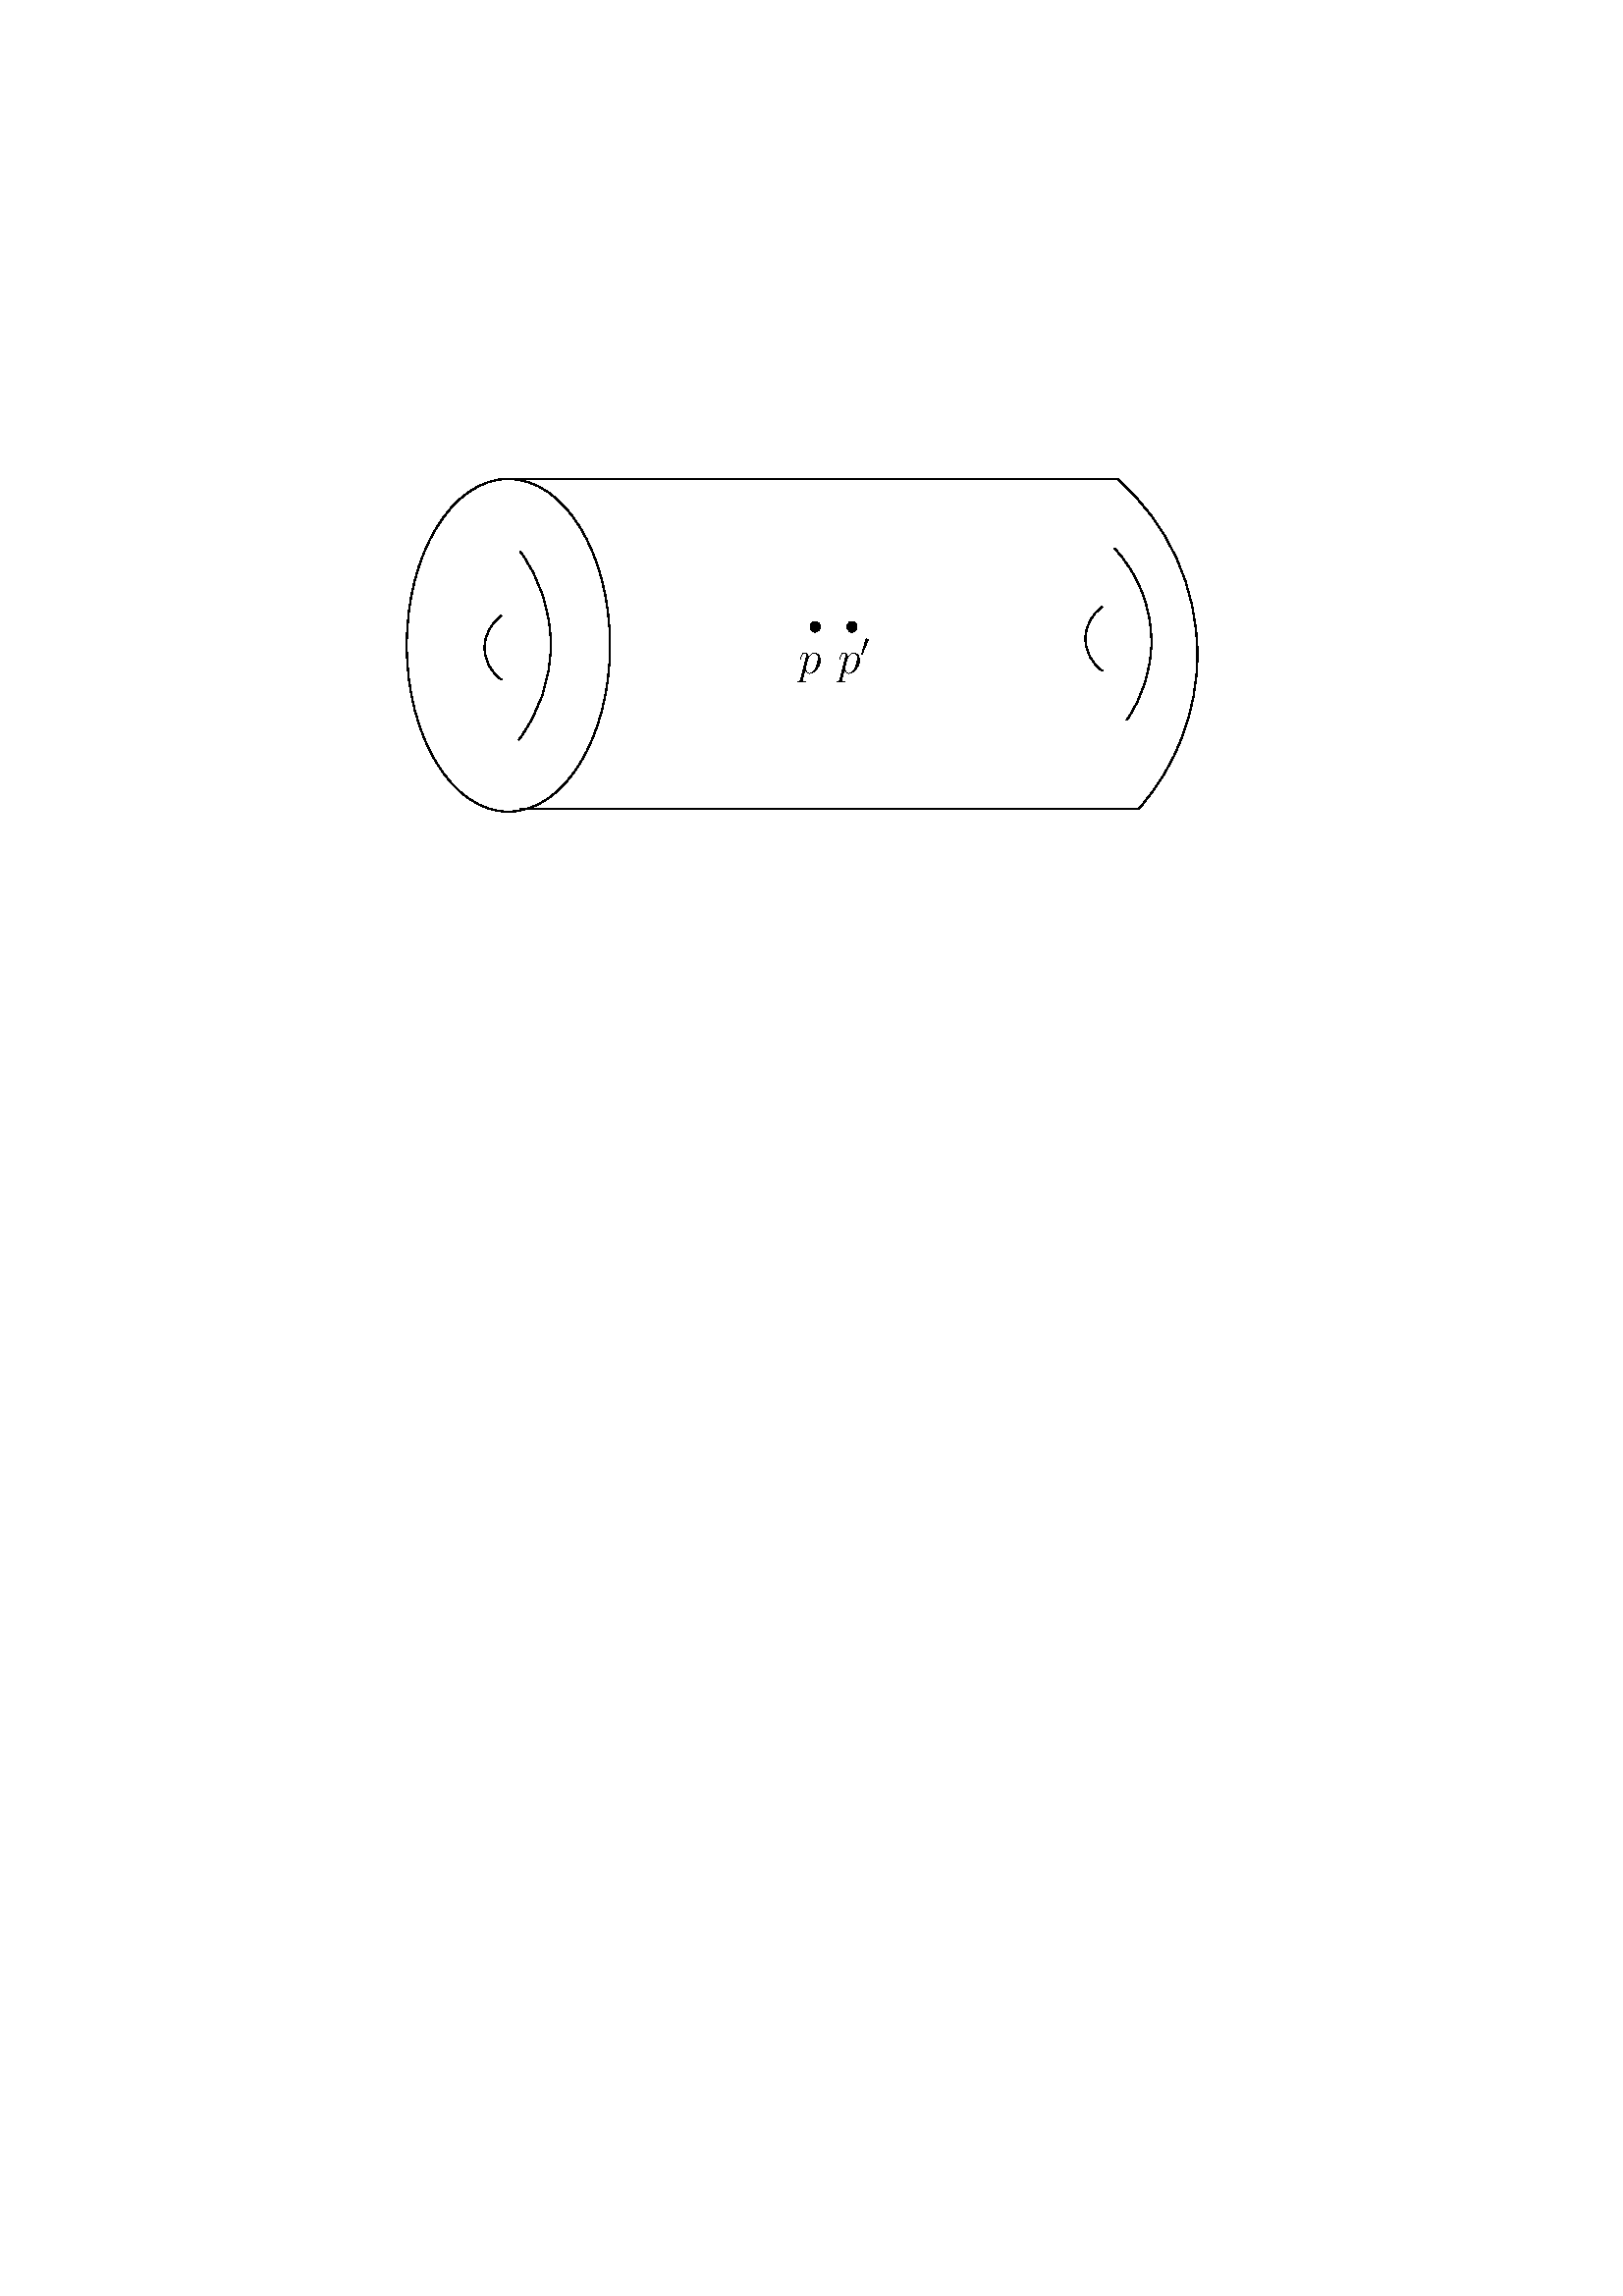
\includegraphics[width=0.75\linewidth]{figures/gla7-9.png}
\caption{A pair of Hecke modifications made at the same value of $z$ but at distinct points in $I$.（原文 Fig.~20）}
\label{fig:xytampo}
\end{figure}

但到此为止我们还没有说到任何依赖于加权射影空间奇点的地方。为看清奇点的作用，令 $^L\negthinspace w=(1/2,-1/2)$ 为对应于二维表示的权。相应的 Wilson 算子与自身的算子乘积展开应当读作
% 式 (10.31)
\setcounter{equation}{30}
\begin{equation}\label{eq:murtog}
T({}^L\negthinspace w)\cdot T({}^L\negthinspace
w)=T({}^L\negthinspace\bar w)\oplus T(0),
\end{equation}
 其中 $0$ 是零权，$T(0)=1$ 是相应的平凡 't Hooft 算子。（系数实际上是某个一维向量空间，但我们把它略去了。）让我们看看这是如何发生的。$^L\negthinspace w$ 型 Hecke 修正的空间同构于 $\Bbb{CP}^1$。若（\xytampo）我们在同一点 $z\in C$、但在 $I$ 中不同点处反复作 $^L\negthinspace w$ 型的 Hecke 修正，就得到模空间 $\bar\EUZ({}^L\negthinspace w,z,y;{}^L\negthinspace w,z,y')$，它是 $\Bbb{CP}^1$ 上的 $\Bbb{CP}^1$ 丛。其上同调是四维的，非零类出现在维数 $d=0,2,2,4$，故 $\EUK$ 的本征值为 $-2,0,0,2$。

现在让我们试着取 $y\to y'$ 的极限。对任意 $y<y'$，我们可以用 Hodge 理论；$\bar\EUZ$ 上调和形式的空间是四维的。在 $y=y'$ 处出现一个 $A_1$ 轨形奇点；局部结构看起来像 $\Bbb{R}^4/\Bbb{Z}_2$。当 $y$ 略小于 $y'$ 时（与区间 $I$ 的长度相比），这个奇点被消解。该消解可在局部用超凯勒流形 $\EUWW$（由 \cite{ref130} 发现）作为模型，它在一个复结构中可以等同于 $T^*\Bbb{CP}^1$。$\EUWW$ 上的度规是完备的，而且在无穷远处渐近于 $\Bbb{R}^4/\Bbb{Z}_2$ 上的平坦度规。

对我们至关重要的是，$\EUWW$ 上 ${\Bbb{L}}^2$ 调和形式的空间是一维的，由一个二形式 $\omega$ 生成 \cite{ref130}。（注意这里 ${\Bbb{L}}^2$ 条件涉及无穷远处的行为，而在相交上同调的定义中它涉及奇点附近的行为。）由于属于 ${\Bbb{L}}^2$，这个形式支撑在例外除子附近；当 $y\to y'$（例外除子收缩）时，它收敛为在奇点处有 delta 函数支撑的形式。它有 $d=2$，故对应于鬼数 $\EUK=0$ 的上同调类，而这个值对应于 $^L\negthinspace G=SU(2)$ 的平凡表示。$\EUWW$ 上这个 ${\Bbb{L}}^2$ 调和二形式之所以存在，是出于可用 \cite{ref131} 中论证理解的拓扑原因。

现在我们可以理解算子乘积关系 \eqref{eq:murtog} 的含义了。左端联系着反复 Hecke 修正的空间 $\bar\EUZ$。当 $y<y'$ 时，它是 $\Bbb{CP}^1$ 上的 $\Bbb{CP}^1$ 丛，有四维的调和形式空间，即物理 Hilbert 空间 ${\cal H}$。这个空间的一个三维子空间由这样的调和形式组成：它们当 $y\to y'$ 时收敛为 $\bar\EUZ{}^*=\Bbb{WCP}^2(1,1,2)$（即 $\bar\EUZ$ 在 $y\to y'$ 时的极限）光滑部分上的 ${\Bbb{L}}^2$ 调和形式。它们反映了 $T({}^L\negthinspace\bar w)$ 对 ${\cal H}$ 的贡献。第四个调和形式在 $y$ 接近 $y'$ 时可用 $\EUWW$ 上的 $\Bbb{L}^2$ 调和形式来近似，并且支撑在例外除子附近。这第四个调和形式的支撑当 $y\to y'$ 时收敛到 $\bar\EUZ{}^*$ 的奇点，而后者是权 $^L\negthinspace w=0$ 的 Hecke 修正空间。它是 $T(0)$ 对 ${\cal H}$ 的贡献。$T(0)$ 的系数为 1，这件事表达了：当 $y\to y'$ 时收敛到奇点的调和二形式空间恰好是一维的。更确切地说，$T(0)$ 的系数就是这个一维的调和形式空间。

更一般地，设给定任意一对权 $^L\negthinspace w$、$^L\negthinspace w'$。我们要描述算子乘积 $T({}^L\negthinspace w)\cdot T({}^L\negthinspace w')$，预期它具有如下形式
% 式 (10.32)
\setcounter{equation}{31}
\begin{equation}\label{eq:mitory}
T({}^L\negthinspace w)\cdot T({}^L\negthinspace
w')=T({}^L\negthinspace\,\bar w)\oplus\left(\oplus_{\alpha\in \EUR'}\,N_\alpha
\otimes T({}^L\negthinspace w_\alpha)\right),
\end{equation}
 其中 $^L\negthinspace\,\bar w={}^L\negthinspace w+{}^L\negthinspace w'$，求和遍历联系到 $^L\negthinspace\,\bar w$ 的各个权。当 $y\to y'$ 时，$\bar\EUZ({}^L\negthinspace w,y,z;{}^L\negthinspace w,y',z)$ 作为空间收敛到 $\bar\EUZ({}^L\negthinspace\,\bar w,y,z)$（后者对 $y$ 与 $z$ 的依赖无关紧要）。模空间上的一些 ${\Bbb{L}}^2$ 调和形式收敛为 $\bar\EUZ({}^L\negthinspace\,\bar w)$ 光滑部分上的这类形式。这些是 $T({}^L\negthinspace\,\bar w)$ 在算子乘积展开中的贡献。另一些则收敛为在 $\bar\EUZ({}^L\negthinspace w_\alpha)$（对 $^L\negthinspace\bar w$ 的某个伴随权 $^L\negthinspace w_\alpha$）上有 delta 函数支撑的形式。当 $y\to y'$ 时支撑在 $\bar\EUZ({}^L\negthinspace w_\alpha)$ 上、而不支撑在任何 $^L\negthinspace w_\alpha$ 的伴随权 $^L\negthinspace w_\beta$ 对应的 $\bar\EUZ({}^L\negthinspace w_\beta)$ 上的那些形式，就是 $T({}^L\negthinspace w_\alpha)$ 在算子乘积中的贡献。

最后，我们简要说明这一想法在数学上是如何表述的 \cite{ref97,ref98}。模空间 $\bar\EUZ({}^L\negthinspace w,z,y;{}^L\negthinspace w',z,y')$ 是纤维为 $\bar\EUZ ({}^L\negthinspace w',z,y')$、底为 $\bar\EUZ({}^L\negthinspace w,z,y)$ 的纤维化，正如我们在第~\ref{sec:kahstr}~节所解释的。当 $y\to y'$ 时，这个模空间被「坍缩」（blown down），以得到更奇异的空间 $\bar\EUZ({}^L\negthinspace\,\bar w,z,y')$，后者对 $z$ 与 $y'$ 的依赖无关紧要。这一坍缩是一个有理映射
% [WARN] 公式 \eqn\eqref{eq:normo} 无编号或重复
\begin{equation*}
\tag*{(10.33)}
\pi:\bar\EUZ({}^L\negthinspace w,z,y;{}^L\negthinspace
w',z,y')\to \bar\EUZ({}^L\negthinspace\,\bar w).
\end{equation*}

我们把 $\bar\EUZ({}^L\negthinspace w,z,y;{}^L\negthinspace w',z,y')$ 上的标准相交上同调复形记作 $IC({}^L\negthinspace w)\star IC({}^L\negthinspace w')$。（该记号的动机来自此空间的纤维丛结构。）相交上同调中有推下映射 $\pi_*$。由于层 $IC({}^L\negthinspace w)\star IC({}^L\negthinspace w')$ 在第~\ref{sec:affgrass}~节所谓的群 $GL(N,{\cal O})$（或其他 $G$ 对应的类似群 $G({\cal O})$）之下不变，而 $\pi_*$ 与该作用交换，所以推下 $\pi_*(IC({}^L\negthinspace w)\star IC({}^L\negthinspace w'))$ 同样在 $G({\cal O})$ 下不变。因此可以把它展开为 $\bar\EUZ({}^L\negthinspace\bar w)$ 的标准相交上同调复形 $IC({}^L\negthinspace\bar w)$ 与那些支撑在带权 $^L\negthinspace w_\alpha$（伴随于 $^L\negthinspace\bar w$）的奇异轨道上的复形 $IC({}^L\negthinspace w_\alpha)$ 之和。（这些是 $\bar\EUZ({}^L\negthinspace\bar w)$ 上仅有的 $G({\cal O})$-不变相交上同调复形。）

于是我们必须有\footnote{我们已把所有复形作维数平移，使其在正维数与负维数之间对称。映射 $\pi_*$ 保持这一对称性。因此我们不必担心进一步的平移。}
% 式 (10.34)
\setcounter{equation}{33}
\begin{equation}\label{eq:yrox}
\pi_*\left(IC({}^L\negthinspace w)\star
IC({}^L\negthinspace w')\right)=IC({}^L\negthinspace\bar
w)\oplus \left(\bigoplus_\alpha\, \tilde N_\alpha \otimes \,IC({}^L\negthinspace w_\alpha)\right).
\end{equation}
 首项 $IC({}^L\negthinspace\bar w)$ 的「系数」是平凡的一维向量空间（可以略去），因为映射 $\pi$ 在模空间的光滑部分上是同构。首项的这个性质在式~\eqref{eq:hffo} 的讨论中有初等的解释。其余的「系数」是向量空间 $\tilde N_\alpha$。这一表述类似于 't Hooft 算子乘积的一般结构 \eqref{eq:hffo}\ 或 \eqref{eq:zurgo}，其中相交复形 $IC({}^L\negthinspace w_\alpha)$ 代表 't Hooft 算子 $T({}^L\negthinspace w_\alpha)$ 的贡献。当然，证明 \cite{ref97,ref98} 的困难部分在于描述空间 $\tilde N_\alpha$，并建立它们与 \eqref{eq:omigron} 中出现的类似空间 $N_\alpha$ 的同构。

\begin{yizhu}[易错点]
按：本片反复出现的「系数」有两种，读时须分清。第~\ref{sec:lineop}~节用 $c$-数系数 $n_\alpha$ 写出的是 Wilson {\it 圈}算子的算子乘积展开（式~\eqref{eq:tryo}）；而静态 Wilson {\it 线}算子处理的是一段带边界的时间演化，其算子乘积展开 \eqref{eq:docus} 的系数是向量空间 $N_\alpha$ 而非整数。二者之间只差一个取迹：把时间方向紧致化为圆、对和乐取迹，$N_\alpha$ 就退化为它的维数 $n_\alpha$。这也解释了拓扑场论中圈算子算子乘积系数恒为整数的来源——那个整数其实是某个向量空间的维数。
\end{yizhu}

\begin{yizhu}[物理图像]
按：「一些有用的膜（Some Useful Branes）」一段的要点是：不必真的去量子化带 't Hooft 算子的四维规范理论，而应把边界条件翻译成二维 sigma 模型的膜。取 $B$ 支撑在 $\EUZ$ 上、固定全纯型 $E_-$ 而让 $\varphi$ 任意，取 $B'$ 支撑在 $\varphi=0$ 的那部分上，两膜横截于 $(E_-,0)$ 一点；于是超对称位形空间恰好就是 Bogomolny 模空间 $\EUZ$。时间分量 $\phi_0$ 在四维理论中是「有质量」的，在 sigma 模型中没有可供指定的边界条件，只能作为源出现在方程中——这正是本片开头要强调「选取合适的膜」的原因。
\end{yizhu}

\begin{yizhu}[易错点]
按：$\bar\EUZ$ 一般带有奇点（单极子冒泡的降权处），因此物理态空间不能取普通 de Rham 上同调，必须用相交上同调；后者（在标准猜想成立的前提下）可粗略地理解为光滑部分的 ${\Bbb{L}}^2$ 上同调，并作 $A$-模型式的维数平移 $\EUK=d-{\rm dim}_{{\Bbb C}}(X)$。物理上真正用到的性质是：$\bar\EUZ$ 的奇点结构不依赖于膜的位置 $p_i$，正因如此，才能用拓扑场论的论证说明 Hilbert 空间与 $p_i$ 无关，也才能把它当作一个只依赖边界条件的向量空间来用。
\end{yizhu}

\begin{yizhu}[物理图像]
按：$y\to y'$ 时出现 $A_1$ 轨形奇点 $\Bbb{R}^4/\Bbb{Z}_2$，它由超凯勒流形 $\EUWW$（Eguchi--Hanson 空间，在某些复结构下即 $T^*\Bbb{CP}^1$）解消；$\EUWW$ 上恰有一个 ${\Bbb{L}}^2$ 调和二形式 $\omega$，它支撑在例外除子附近，当例外除子收缩时收敛为奇点处的 delta 形式。$\omega$ 的次数为 $2$，故鬼数为 $0$，对应于 $^L\negthinspace G=SU(2)$ 的平凡表示，这正解释了 \eqref{eq:murtog} 中 $T(0)$ 的系数为何是 $1$。注意「${\Bbb{L}}^2$」在两处含义不同：在相交上同调的定义中它约束奇点附近的行为，而在 $\EUWW$ 上它约束的是无穷远处的行为。
\end{yizhu}

\begin{yizhu}[原文疑误]
按：「相应的 Wilson 算子与自身的算子乘积展开应当读作」一句，原文作 “the corresponding Wilson operator”，但紧随其后的式~\eqref{eq:murtog} 左端是 $T({}^L\negthinspace w)\cdot T({}^L\negthinspace w)$、右端首项是 $T(0)$，全段讲的都是 't Hooft 算子；Wilson 算子在这里只是作为电磁对偶的对照物出现。故此处应读作「相应的 't Hooft 算子」。译文照录原文的用词，并在此标出。
\end{yizhu}

\begin{yizhu}[易错点]
按：片中有两条单独成行的文献引用（分别指向相交同调理论的经典文献），位于「首先，该定理所用的上同调理论是相交上同调」之前。这是原文排版中的引用行，并非排版错误，已原样保留在两段之间，其命令与位置均未改动。
\end{yizhu}

\begin{yizhu}[含糊点拨]
按：数学上 \eqref{eq:yrox} 的推下与展开正是 Lusztig、Ginzburg、Mirković--Vilonen 的相交上同调卷积（即本片末尾所引的三项工作）：两两相交复形的卷积被推下后，按 $G({\cal O})$-不变性分解为各 $IC({}^L\negthinspace w_\alpha)$ 之和，系数即向量空间 $\tilde N_\alpha$。真正困难的部分不是这个分解形式，而是证明 $\tilde N_\alpha$ 同构于 \eqref{eq:omigron} 中的 $N_\alpha$——那才是几何 Satake 对应与张量积分解在数学上的等号内容。
\end{yizhu}
